\chapter{Laser\label{chapter:laser}}
\lhead{Laser}
\begin{refsection}
\chapterauthor{Arwed Schudel und Claudio Stucki}


\section{Einleitung}

Der Begriff Laser stammt aus dem Englischen und steht f"ur 
"{}Light Amplification by Stimulated Emission of Radiation"{}.
Auf Deutsch bedeutet Laser Licht-Verst"arkung durch stimulierte Emission 
von Strahlung. Dieser Name wird f"ur das Ger"at, welches Laserstrahlen erzeugt 
als auch f"ur den physikalischen Effekt verwendet. Der Begriff Laser wird
ebenfalls f"ur eine Segelbootsklasse und f"ur ein Automodell von Ford
verwendet,
jedoch hat dies nichts mit unserer Arbeit zu tun.

Laserstrahlen sind elektromagnetische Wellen,
welche in einer extrem hohen Intensit"at und sehr engem
Frequenzbereich geb"undelt werden. Diese Art wird als monochromatisches
Licht bezeichnet, da genau eine Wellenl"ange ausgesendet wird. 
Durch diese Eigenschaften ist es m"oglich, extrem kurze und
intensive Strahlenimpulse "uber eine l"angere Distanz zu "ubermitteln,
welche zum Beispiel bei der Nachrichtentechnik eingesetzt werden.

Ausserdem k"onnen mittels Laser grosse Energiemengen ber"uhrungslos
"ubertragen werden, Diese Eigenschaft wird unter anderem bei Schneid-
und Schweisswerkzeugen eingesetzt. Deshalb sind starke Laserstahlen auch 
sehr gef"ahrlich, insbesondere f"ur die Augen, da der Laser auf der Netzhaut
gef"ahrliche Verbrennungen verursachen kann.

Die Lasertechnologie wird in fast allen Branchen sowie im Alltag verwendet, 
sei es als einfacher Lichtzeiger (z.B bei Pr"asentationen),
zum Drucken von Dokumenten oder um von einer CD Musik zu h"oren. 
Weitere Anwendungsgebiete sind von Entfernungsmessger"ate, 
Gravierger"ate bis hin zu medizinischen Lasern und Sicherheitsanwendungen
(Lichtschranken).

Mit Hilfe des Lasers ist es m"oglich elektromagnetische Wellen im Spektrum
von Infrarot "uber sichtbares Licht, bis zu ultraviolettem Licht und 
R"ontgenstrahlen herzustellen. F"ur die Farbe des Lasers sind 
verschiedenen Materialien verantwortlich. Ebenfalls ist es m"oglich mittels 
Laserprinzip Mikrowellen auszusenden, dieses Produkt wird jedoch Maser genannt.


\subsection{Geschichte}

Der Effekt der stimulierten Emission wurde bereits 1916 vom bedeutenden 
Physiker Albert Einstein entdeckt. Jedoch erst 13 Jahre sp"ater gelang der 
experimentelle Nachweis durch Rudolf Ladenburg. Die Forschung wurde durch 
Theodore Maiman vorangegetrieben, welcher 1960 den ersten Laser 
fertigstellte. Von der Entdeckung bis zum ersten Fertigprodukt dauerte es 
fast 50 Jahre. Dieser Rubinlaser war ein Feststofflaser (Kristall). Sp"ater 
wurden Gaslaser und Fl"ussiglaser entwickelt. Die Halbleiter-Laserdioden, 
welche langlebiger sind und wir aus dem CD-Player kennen, wurden erst in den 
sp"aten 1980er Jahren entwickelt.


\section{Aufbau eines Lasers}

Die wichtigsten Bestandteile eines Laser sind das Lasermedium, die Pumpe so 
wie der Resonator. Der Laserstrahl wird in einem Lasermedium erzeugt und 
durch den optischen Resonator mit Hilfe von zwei Spiegeln in die richtige 
Form gebracht. 

Die Laserpumpe ist daf"ur verantwortlich, dass die Atome oder Molek"ule auf 
ein neues h"oheres Energielevel gebracht werden. Durch das Hineinpumpen von 
zus"atzlicher Energie, elektrische Energie, 
zum Beispiel Gleichstrom bei einer Laserdiode, Licht oder 
Gasentladung, wird das Lasermedium aus dem thermodynamischen Gleichgewicht 
geholt und der Wechsel der Energieniveaus beginnt. Die Pumpe bringt die 
Molek"ule oder Atome vom Grundzustand in einen angeregten Zustand. Dadurch 
wird eine Besezungsinversion erreicht und der Laser beginnt zu leuchten. Wie 
die Zustandswechsel von statten gehen und wieviele Enegieniveaus vorhanden 
sein m"ussen, wird im Kapitel \ref{Wechselwirkung} genauer erkl"art.

Das Lasermedium ist das aktive Medium, in welchem ein "Ubergang angeregter 
Molek"ule oder Atome in einen energetisch g"unstigeren Zustand statt findet. 
Bei diesem Vorgang wird ein Photon, welches wir als Licht wahrnehmen, 
freigesetzt. Das Medium wird vor allen durch den Aggregatzustand 
unterschieden und kann fest (z.B Halbleitermatrial, Kristalle), fl"ussig (z.B 
Farbstoffl"osungen) oder gasf"ormig (z.B $CO_{2}$, He-Ne, Sauerstoff oder 
Stickstoff) sein. Das Lasermedium ist verantwortlich f"ur die Farbe, 
respektive die Wellenl"ange, welche einen Laser aussendet.

Der Laserresonator ist daf"ur verantwortlich, dass nur Photonen mit 
einer bestimmten Wellenl"ange $\nu$ und einer bestimmten Energie $h\nu$ 
das Lasermedium verlassen. Somit verlassen nur identische Photonen das 
Lasermedium. Dies wird mit Hilfe von zwei verschiedenen Spiegeln 
erreicht. Der erste reflektiert alle ankommenden Photonen und regt 
dadurch die stimulierte Emission zus"atzlich an. Der zweite Spiegel ist 
teilduchl"assig und l"asst nur Photonen mit der richtigen Intensit"at 
und Energie durch. Dadurch entsteht ein konstanter Laserstrahl.

Je nach Produkt wird der Laserstrahl mit einer Sammellinse geb"undelt, 
was insbesondere bei der Laserdiode sehr wichtig ist.

\begin{figure}
\center
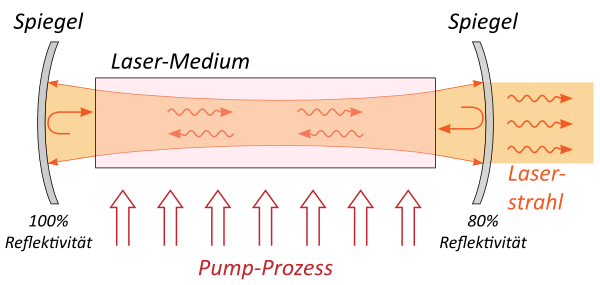
\includegraphics[width=7cm]{laser/bilder/aufbau.png}
\caption{Bestandteile eines Laser \cite{Aufbau}}
\label{Laser Aufbau}
%Quelle https://lp.uni-goettingen.de/get/text/5344
\end{figure}


\section{Wechselwirkung mit Strahlung}
\label{Wechselwirkung}
Die Atome befinden sich auf unterschiedlichen Energieniveaus. 
Nun gibt es verschiedene Prozesse die dieses Energieniveau "andern k"onnen.
In diesem Kapitel werden genau diese Prozesse beschrieben und erkl"art und
bildlich dargestellt.


\subsection{Spontane Prozesse}
\label{Spontane Prozesse}
%Quelle: LP_WS_09_10_Zusammenfassung_Laserprinzip.pdf
Die Atome befinden sich in einem angeregten Zustand mit einer Energie $E_2$. 
Diese Atome k"onnen durch die Abgabe eines Photons auf ein tieferes
Energieniveau $E_1$ gelangen.
Dieser Wechsel des Energieniveaus findet spontan und v"ollig unabh"angig vom
"auseren Strahlungsfeld statt.
Deswegen wird dieser Prozesse als spontane Emissionen bezeichnet.

Die Richtung, die Phase und auch die Polarisation der abgestrahlten
elektromagnetischen Welle ist dabei rein zuf"allig.
Hingegen kann die "Ubergangswahrscheinlichkeit des Vorgangs von $E_2$ nach
$E_1$ mit dem Einsteinkoeffizienten $A_{21}$ angegeben werden.
Siehe Abbildung \ref{spontane Emission}

Das abgegebene Photon hat eine Energie von $\Delta E = E_2 - E_1$.
Die Frequenz des Photons $(\nu)$ ist dabei proportional zur Energie:
\[ \Delta E = h\cdot \nu\]
Spontane "Uberg"ange finden nur von energetisch h"oheren Energieniveaus in
tiefer liegende Niveaus statt.

\begin{figure}
\centering
\includegraphics[width = 6cm]{laser/niveau-3.pdf}
\caption{spontane Emission}
\label{spontane Emission}
\end{figure}


\subsection{Stimulierte Prozesse}
Die stimulierten Prozesse brauchen im Gegensatz zu den spontanen
Prozessen (Kapitel \ref{Spontane Prozesse}) ein "ausseres Strahlungsfeld.
Dadurch stimmen die Phase, die Frequenz sowie die Polarisation mit dem
"ausseren Feld "uberein.
Auch die stimulierten Prozesse werden durch den Einsteinkoeffizient angegeben.
Dieser wird dabei mit dem Buchstaben $B$ angegeben.
Findet ein "Ubergang vom h"oheren Energieniveau auf ein tieferes statt,
so spricht man von einer Emission. Dabei wird ein Photon ausgesendet.
Der umgekehrte Vorgang ist die Absorption, dabei wird ein Elektron absorbiert
und das Atom besitzt anschliessend eine h"ohere Energie.


%--------------------------------------------------------------------
\subsubsection{Stimulierte Emission}

Dabei erzeugt ein eintreffendes Photon einen "Ubergang vom h"oheren Niveau
$E_2$ ins $E_1$. 
Bildlich gesprochen zieht es ein zweites Photon mit sich.
Das freigewordene Photon hat eine Energie von $E_2 - E_1$.
Diese beiden Photonen haben identische Eigenschaften.
Dieser Vorgang erlaubt die Lichtverst"arkung, den grundlegenden Prozess jedes
Lasers.

Die Wahrscheinlichkeit, mit dem so ein Energieniveauwechsel von $E_2$ nach
$E_1$ stattfindet, ist proportional zum Einsteinkoeffizient $B_{21}$.
Dieser Prozess ist in der Abbildung \ref{Stimulierte Prozesse} links bildlich
dargestellt.

\subsubsection{Stimulierte Absorption}
Bei der Absorption werden Photonen mit einer spezifischen Energie absorbiert.
Dabei steigt die Energie des Atomenes aus dem tieferen Zustand in den
h"oheren.
Die Energiedifferenz der Atomenergien betr"agt dabei genau der Energie des
Photons.
Mit dem Einsteinkoeffizient $B_{12}$ wird ein Mass f"ur die
Wahrscheinlichkeit angegeben, dass eine Energieniveauwechsel von $E_1$ nach
$E_2$ stattfindet.
Dieser Prozess ist in der Abbildung \ref{Stimulierte Prozesse} rechts bildlich
dargestellt.

\begin{figure}
\centering
\includegraphics[width = 12cm]{laser/niveau-6.pdf}
\caption{Stimulierte Prozesse}
\label{Stimulierte Prozesse}
\end{figure}


\subsection{Einsteinkoeffizienten $B_{21}$ = $B_{12}$}
\label{B21=B12}
Die Einsteinkoeffizienten $B_{21}$ und $B_{12}$ m"ussen gleich gross sein.
Dies folgt aus der quantenmechanischen Theorie, welche besagt, dass der
Hamilton-Operator symmetrisch ist:

%ungest"ohrte und gest"ohtre Hamiltonmatrix
\[
H =\begin{pmatrix}
E_1 & 0  \\
0   & E_2 \\
\end{pmatrix}
+ I\cdot \begin{pmatrix}
b_{11} & b_{12}  \\
b_{21} & b_{22} \\
\end{pmatrix}
=\begin{pmatrix}
E_1+ I\cdot b_{11} & I\cdot b_{12}  \\
I\cdot b_{21} & E_2+I\cdot b_{12} \\
\end{pmatrix}
\]
Die dargestellte Hamilton-Matrix besteht aus dem ungest"orten Teil und 
dem Produkt der Intensit"at und dem Strahlungsfeld im Resonator.
Damit diese Matrix symmetrisch sein kann ist es unumg"anglich, dass $b_{12}$
und $b_{21}$ gleich gross sind.
Somit m"ussen auch die Einsteinkoeffizienten $B_{12}$ und $B_{21}$ "aquivalent
sein.
Da diese Einsteinkoeffizienten ein Mass f"ur die Wahrscheinlichkeit der
stimulierten Vorg"ange sind, hat das Auftreten der stimulierten Emission und
der stimulierten Absorption die selbe Wahrscheinlichkeit.

\subsection{Besetzungsinversion}
\label{Besetzungsinversion}
Damit der Laser seine Photonen aussenden kann, er also "{}lasern"{} kann,
muss die Anzahl der stimulierte Emissionvorg"angen wesentlich gr"osser sein,
als die der stimulierten Absorption.
Weil diese Vorg"ange dieselbe Auftretenswahrscheinlichkeit haben,
muss die Anzahl Atome im h"oheren Energieniveau $E_2$ gr"osser sein,
als die der Atome im $E_1$.
Nur so kann sichergestellt werden, dass der Laser stets mehr stimulierte
Emissionsvorg"ange als stimulierte Absortionsverg"ange hat. 
Dies wiederum ergibt die notwendigen Photonen, die den Laser zum leuchten
bringen.
Ohne diese Besetzungsinversion kann kein Laser funktionieren. 
Dies ist somit die Grundlage jedes Lasers. 
Wie diese Besetzungsinversion zustande kommt ist je nach Laser
unterschiedlich.


\section{2-Niveau System}
\label{2-Niveau System}
\begin{figure}
\centering
\includegraphics[width = 10cm]{laser/niveau-1.pdf}
\caption{2-Niveau Laser}
\label{2-Niveau Laser Meta}
\end{figure}
Bei einem 2-Niveau System sind zwei verschiedene Energieniveaus vorhanden.
Das Energieniveau $E_1$ und das um $\Delta E$ h"oher liegende $E_2$.
Zwischen diesen beiden Niveaus k"onnen die beschriebenen Vorg"ange spontane
Emission, stimulierte Emission und die stimulierte Absorption stattfinden.
Diese sind in der Abbildung \ref{2-Niveau Laser Meta} aufgezeigt.

\subsection{Ratengleichungen}
\label{2-Niveau Ratengleichungen}
Die Ratengleichungen beschreiben die Ver"anderung der Anzahl Atome in den
einzelnen Energieniveaus.
Anhand der Abbildung \ref{2-Niveau Laser Meta} ist die Interpretation der
Ratengleichungen einfach nachvollziehbar.
Die Elemente in den Ratengleichungen sind wie in der Abbildung von links
nach rechts aufgelistet.
\[ \frac{dN_1}{dt} = -\frac{dN_2}{dt} = 
\underbrace{+ B_{21} \cdot  I \cdot N_2}_{\text{Stimuliete~Emission}}
\underbrace{+ A_{21}\cdot N_2}_{\text{Spontane~Emission}}
\underbrace{-B_{12} \cdot I \cdot N_1}_{\text{Stimulierte~Absorption}}\]
Da die Teilchen nur zwischen den zwei Niveaus wechseln k"onnen, ist die Zunahme
von $N_1$ gleich der Abnahme von $N_2$. 
Dies bedeutet zudem, dass $N = N_1 + N_2 $ immer konstant ist.
Damit nun ein Laser Lichtwellen aussenden kann, m"ussen stets mehr Atome auf
dem h"oher liegenden Niveau sein.
Dies ist in Kapitel \ref{Besetzungsinversion} erl"autert.
Somit muss die Differenz $\Delta N = N_1 - N_2$ negativ sein.
Die Ableitung der Differenz $\Delta N$ lautet wie folgt:
\[ \frac{d(N_1 - N_2)}{dt} = \frac{d \Delta N}{dt} = -2\cdot B\cdot I\cdot
\Delta N + A\cdot N - A\cdot \Delta N \]
Aus dieser Differentialgleichung kann nun bewiesen werden, dass dies bei einem
Dauerstrich-Laser mit nur 2 Energieniveaus nie der Fall sein kann. 
F"ur den station"aren Zustand in dem der Laser sein Licht aussenden soll, muss
die Differentialgleichung 0 werden.
Diese nun nach $\Delta N$ aufgel"ost ergibt:
\[ \Delta N = \frac{A\cdot N}{A+2\cdot B\cdot I} = \frac{N}{1+2\cdot I 
\frac{B}{A}} \stackrel{!}{>} 0\]
Da alle in dieser Gleichung vorkommenden Elemente $N$, $I$, $A$ und $B$ immer positiv
sind, ist auch das Ganze positiv.
Das ist somit auch der Beweis, das ein Laser mit 2 Energieniveaus nicht als
Laser funktionieren kann.
\begin{figure}
\centering
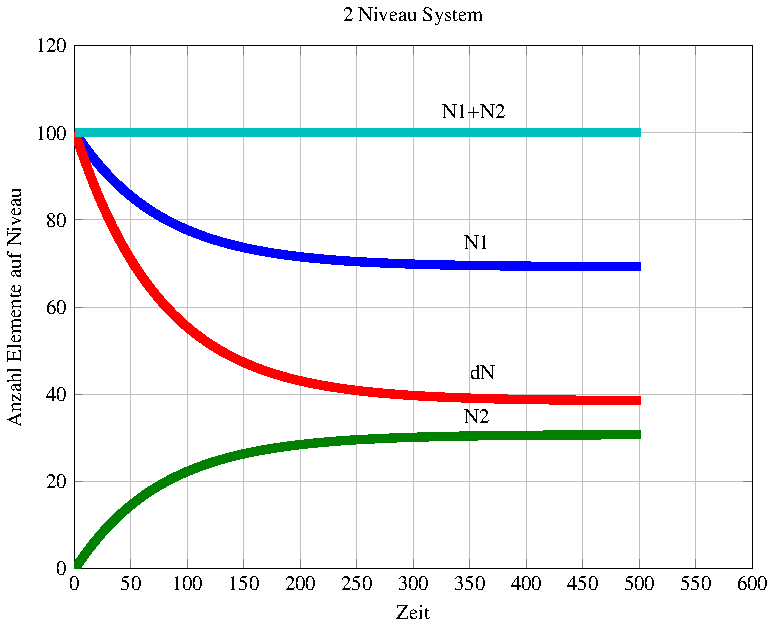
\includegraphics[width = 10cm]{laser/bilder/2_niveau.pdf}
\caption{2-Niveau Laser}
\label{2-Niveau Laser}
\end{figure}

\subsection{Simulation}
\label{2-Niveau System Simulation}
Mit den Gleichungen  $\frac{dN_1}{dt} = -\frac{dN_2}{dt}$ ist mit Hilfe von
Matlab / Simulink numerisch eine Simulation druchgef"uhrt worden.
Diese ist in Abbildung \ref{2-Niveau Laser}  dargestellt.
Die wichtigste Kurve ist dabei $\Delta N $ 
(in der Abbildung \ref{2-Niveau Laser} mit $dN$ angeschrieben)
die immer positiv ist.
Zur Erinnerung, f"ur einen Dauerstrich-Laser m"usste eine Besetzungsinversion
(Kapitel \ref{Besetzungsinversion}) erfolgen.
Dies w"are der Fall, wenn die $\Delta N $ - Kurve negativ ist.
Somit best"atigit die Simulation die Erkenntnis aus Kapitel
\ref{2-Niveau Ratengleichungen}, dass ein Dauerstrich-Laser nicht
funktionieren kann.

\section{3-Niveau System}
\label{3-Niveau System}

\begin{figure}
\centering
\includegraphics[width = 10cm]{laser/niveau-2.pdf}
\caption{3-Niveau Laser}
\label{3-Niveau Laser}
\end{figure}

In diesem System gibt es ein drittes Niveau $E_3$ mit einer h"oheren Energie
als $E_2$. 
Der Energieunterschied zwischen $E_1$ und $E_2$ ist gr"osser 
als $E_2$ und $E_3$.
Zu Beginn des Laservorganges sind die allermeisten Atome im Grundniveau $E_1$.
Durch die Pumpe werden die Atome in das h"ochste Energieniveau $E_3$
transportiert.
Dort bleibt sie nur sehr kurzzeitig, bevor sie mittels spontaner Emission auf das
Niveau $E_2$ herunterfallen.
Dort bleibt sie wesentlich l"anger als zuvor auf $E_3$.
Der Zeitpunkt an dem die Anzahl der Atome auf dem Niveau $E_2$ gr"osser ist als
$E_1$ wird Besetzungsinversion (Kapitel \ref{Besetzungsinversion}) bezeichnet.
Genau von diesem Zeitpunkt an sendet der Laser seinen Lichtstrahl aus.

\subsection{Ratengleichungen}
\label{3-Niveau Ratengleichungen}
Die folgenden Gleichungen  beschreiben, wie schon beim 2-Niveau Laser, die
Ver"anderung der drei Energieniveaus.

Die in der Abbildung \ref{3-Niveau Laser} mit $A_{ij}$ beschrifteten
Einsteinkoeffizienten beschreiben die spontanen Emissionen die vom
Energieniveau $E_i$ ins tiefere Energieniveau $E_j$ stattfinden.
Mit $B_{ij}$ werden die Einsteinkoeffizienten der stimulierten Prozesse
vom Energieniveau $E_i$ ins Energieniveau $E_j$ beschrieben. 
Ist der Index $i > j$ so findet eine stimulierte Emission statt,
andernfalls eine stimulierte Absorption.
Wie bei den Ratengleichungen des 2-Niveau Systems sind die Einsteinkoeffienten
mit den Indizes $ij$ und $ji$ gleich.


\begin{align*}
\frac{dN_1}{dt} &=
N_2  A_{21} 
+ N_3 \cdot  A_{31}
+ (N_2 - N_1) \cdot B_{21}\cdot  I_{12}
+ (N_3 - N_2) \cdot B_{31}\cdot  I_{13}\\
\frac{dN_2}{dt} &=
N_3 \cdot  A_{32} 
- N_2 \cdot  A_{21}
- (N_2 - N_1) \cdot  B_{21}\cdot  I_{12}
+ (N_3 - N_2) \cdot  B_{32}\cdot  I_{23}\\
\frac{dN_3}{dt} &=
- N_3 \cdot  A_{32}
- N_3 \cdot  A_{31}
- (N_3 - N_1) \cdot  B_{31}\cdot  I_{13}
- (N_3 - N_2) \cdot  B_{32}\cdot  I_{23}
\end{align*}


Diese drei Differenzialgleichungen lassen sich analog zu den einfacheren
2-Niveau System Gleichungen herleiten.

\subsection{Simulation}
\label{3-Niveau Simulation}
Mit einer Matlab / Simulink-Simulation kann das Verhalten des Lasers anhand
dieser 3 Gleichungen simuliert werden.
Die Wahl der einzelnen Parameter ist jedoch von entscheidender Bedeutung.
Hier wurden sie so gew"ahlt, dass die einzelnen Vorg"ange gut ersichtlich sind.
Das Resultat dieser Simulation ist in der Abbildung
\ref{Simulation 3-Niveau System} ersichtlich.
Die mit $Ni$ beschrifteten Kurven stellen die Besetzung der Energieniveaus
$E_i$ dar.
Der Zeitpunkt der Besetzungsinversion ist ersichtlich, wenn die beiden Niveaus
$N1$ und $N2$ sich kreuzen.
Der Laser funktioniert nun ununterbrochen bis diese Besetzungsinversion
nochmals eintritt.
Das erfolgt erst, wenn die Pumpe ausgeschaltet wird.
In der Simulation ist die Zeit, in welcher der Laser aktiv, ist orange
hinterlegt.

\begin{flushleft}
\begin{figure}
\centering
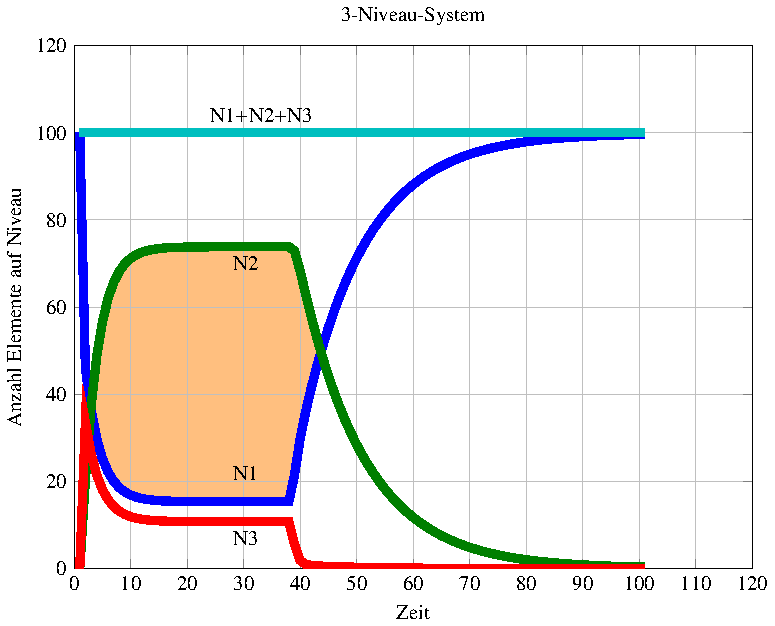
\includegraphics[width = 10cm]{laser/bilder/3_niveau.pdf}
\caption{Simulation 3-Niveau System}
\label{Simulation 3-Niveau System}

\end{figure}
\end{flushleft}

\section{Laserdiode}
\label{Laserdiode}

\subsection{Unterschied Laser - LED}
\label{Unterschied Laser - LED}
Das Licht eines Lasers und einer LED sehen auf den ersten Blick gleich aus.
Bei genauerem betrachten treten aber entscheidende Unterschiede auf.
Der Lichtstrahl einer LED leuchtet sehr hell, beinhaltet dabei aber mehrere
Frequenzanteile des Lichtes.
Bei einem Laser gibt es bekanntlich nur eine Frequenz,
somit auch nur eine Farbe.
Dies kann mit Hilfe eines Prismas nachgewiesen werden.
Dabei n"utzt man die unterschiedlichen Brechungen der einzelnen Frequenzen.
Der zweite grosse Unterschied betrifft die Phase der Lichtwellen.
Diese sind bei der LED willk"urlich und keineswegs immer gleich.
Beim Laser sind diese Lichtwellen immer in Phase.
Dies wird durch die stimulierte Emission erreicht.

Dies wird sichtbar, wenn man den Lichtstrahl einer Lichtquelle
auf einer Oberfl"ache abbildet.
z"undet. Bei der LED wird lediglich ein einziger relativ grosser Punkt 
sichtbar. Beim Laser werden viele kleine Punkte sichtbar, welche in der
Fachsprache Speckles genannt werden. Diese widerspiegelt das koh"arente Licht
des Lasers.

\begin{figure}
\centering
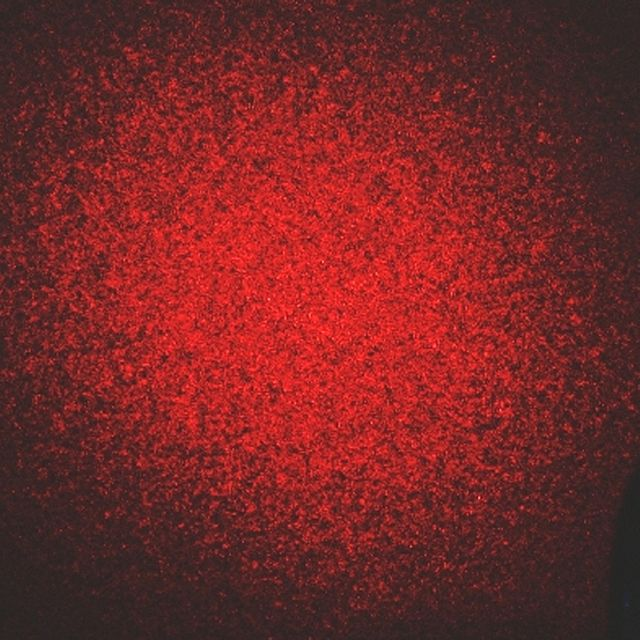
\includegraphics[width = 5cm]{laser/bilder/Objective_speckle.jpg}
\caption{Rote Speckles eines Lasers \cite{WikiSpeckle}}
\index{speckles}
\end{figure}

\subsection{Funktion}
Mit Hilfe einer Leuchtdiode (LED) ist es m"oglich Licht im Spektrum von 
Infrarot bis Ultraviolet herzustellen. Eine Leuchtdiode hat die elektrischen 
Eigenschaften einer Halbleiter-Diode, welche zus"atzlich Licht emittiert. Die 
LED funktioniert nur in Durchlassrichtung, dabei wandern die 
Defektelektronen(L"ocher) von der p-dotierten Seite zum p-n-"Ubergang.Die 
Elektronen wandern von der anderen Seite, der n-dotierten zum p-n-"Ubergang. 
Da die Elektronen ein h"oheres Energieniveau haben, fallen diese in die 
L"ocher hinein und geben dadurch ihre Energie in Form eines Photons (Licht) 
ab. Dieser Effekt wird als Rekombination bezeichnet. Die Lichtfarbe ist von 
den verwendeten Materialien sowie von der Dotierung abh"angig.

Im Gegensatz zur LED, welche die Lichtstrahlen in einem grossen Spektrum im 
Verh"altnis zum Laser abgibt, wird bei beim Laser mittels scharf definierten 
Laser-"Ubergangs nur eine Wellenl"ange ausgestahlt.  
Bei der LED fehlt die Koh"arenz der Strahlung, da 
diese durch die stimulierte Emisson und den Resonator entsteht. Beide 
Voraussetzung sind bei der LED nicht gegeben. 

Eine Laserdiode ist die Weiterentwicklung des LED-Prinzips. Dazu sind jedoch 
noch zwei zus"atzliche Eigenschaften notwendig. Als erstes muss die vorhandene 
spontane Emission, welche ausschliesslich bei LEDs vorkommt, von der 
stimulierte Emission deutlich "ubertroffen werden. Die dazu n"otige 
Besetzungsinversion wird mit einer aktiven Zone zwischen zwei sehr hoch 
dotierten p respektive n Schicht erreicht. Befindet sich die Laserdiode in 
einer Besetzungsinversion (mehr Teilchen sind im h"oheren Energiezustand $E_2$ 
als im energetisch niedrigeren Zustand $E_1$) wird die stimulierte Emission zum 
dominierenden Strahlungsprozess. Dieser Zustand wird erreicht, indem ein 
elektrischer Gleichstrom in Durchlassrichtung als Pumpe dient, welche immer 
f"ur Nachschub von Elektronen und L"ocher sorgt. Als zweites d"urfen die 
Verluste nicht gr"osser sein, als die Produktion der Photonen.
Dies wird mit Hilfe des Resonator erreicht.
Wie beim normalen Laser besteht der Resonator aus teilreflektierenden 
und reflektierenden Spiegel an den Endfl"achen.

Oft befindet sich nebst der Laserdiode auch noch eine Photodiode im gleichen 
Geh"ause, welche n"otig ist, um eine Regelung aufzubauen. Dank der Regelung 
ist die Intensit"at des Laserstrahls immer konstant. Es ist jedoch auch 
m"oglich die Laserdiode mittels konstanten Strom zum leuchten zu bringen. Zum 
Aufbau einer Laserdiode geh"ort ebenfalls eine Linse, welche die Strahlen 
b"undeln. Ohne Linse gibt die Diode einen breiten F"acher ab. Bei st"arkeren 
Laserdioden ist meistens ein K"uhlk"orper im selben Geh"ause befestigt, um 
eine lange Lebensdauer sowie einen konstanten Laserstrahl garantieren zu 
k"onnen. 
\begin{figure}
\centering
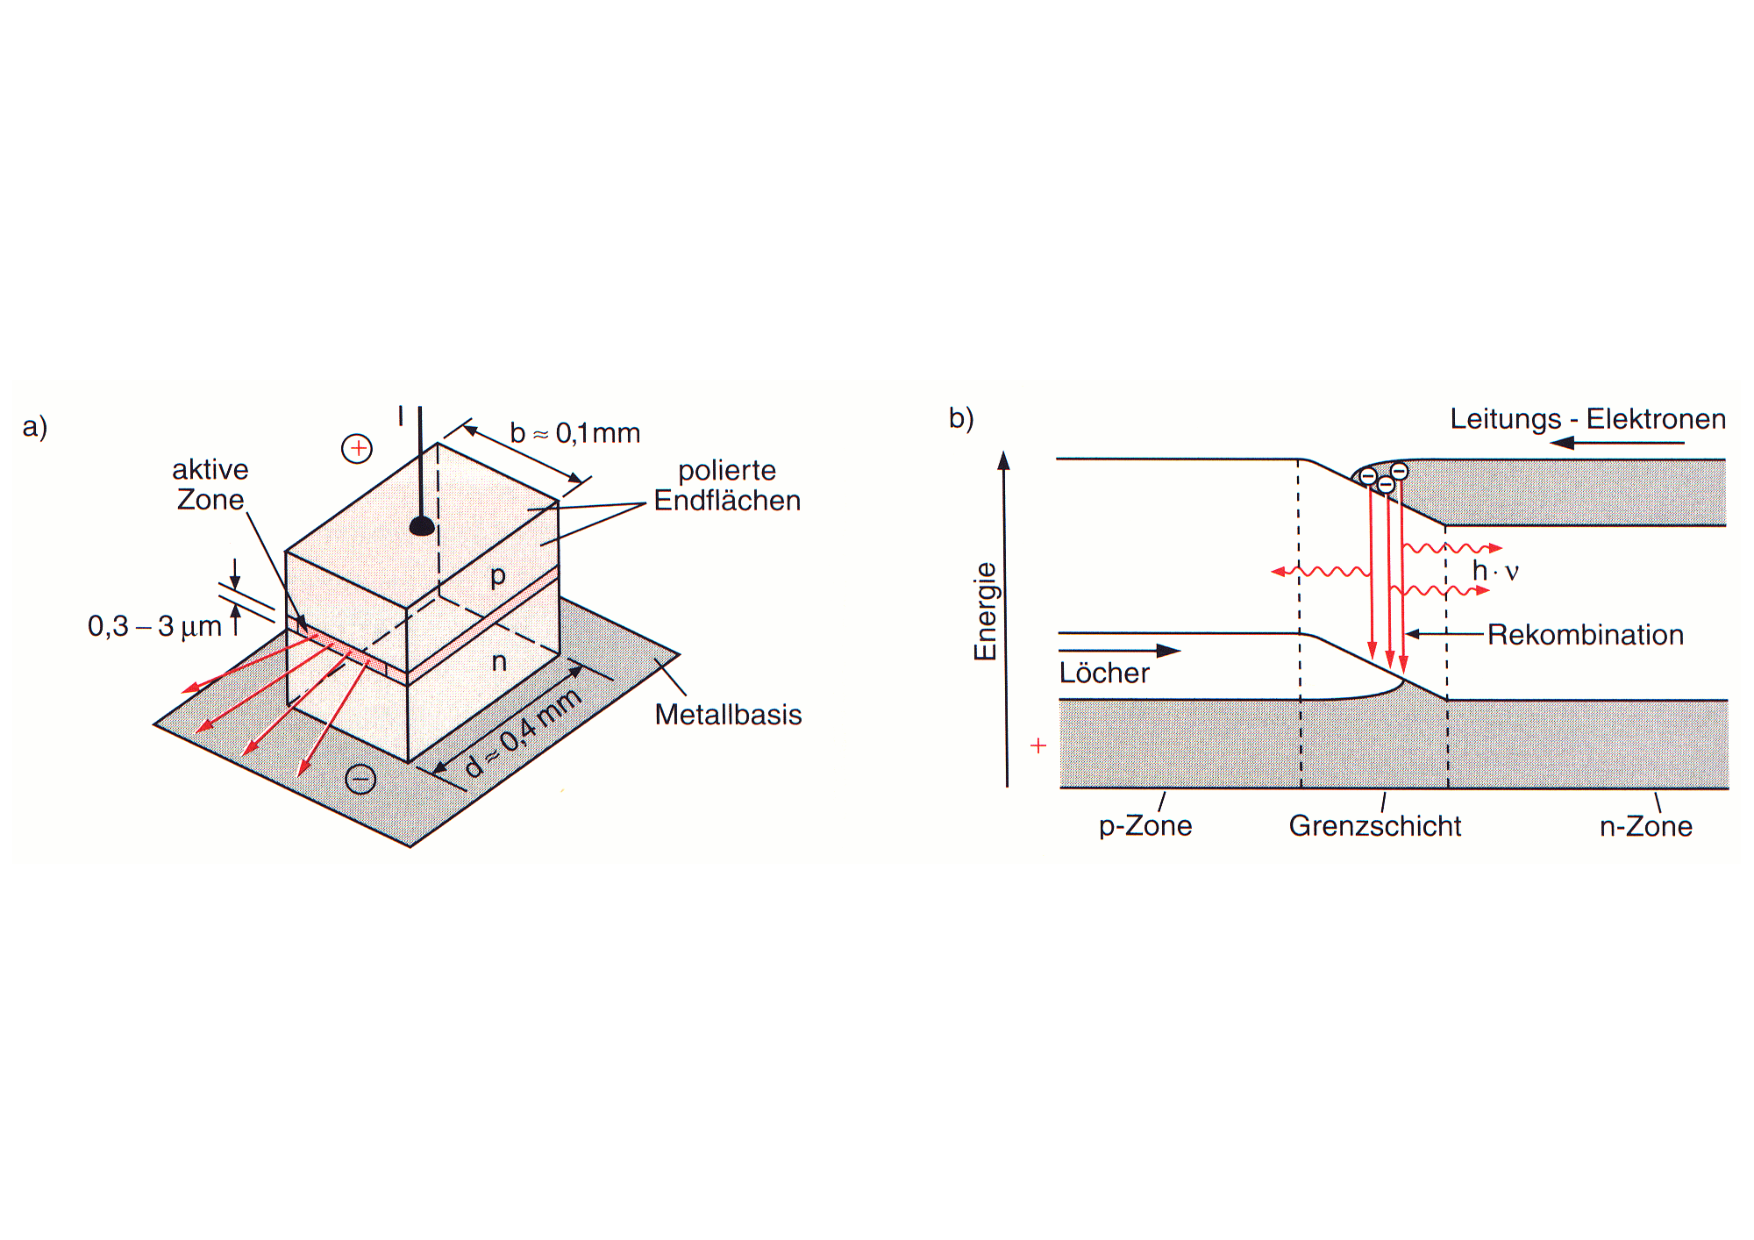
\includegraphics[scale=0.35]{laser/bilder/laserdiodeb.pdf}
\caption{Aufbau und Energieniveaus einer Laserdiode \cite{halbleiterlaser}}
\label{fig:Laserdiode}
\end{figure}

\subsection{Versuch}

Um die Theorie nachzuvollziehen haben wir eine 5 mW Laserdiode im Labor kurz 
unter die Lupe genommen. Wir haben eine Laserdiode an einer konstanten 
Spannungsquelle angeschlossen und mittels Vorwiderstand den Strom 
begrenzt. Dabei haben wir den Strom durch die Laserdiode, die Spannung "uber 
der Diode, sowie der Strom welcher durch die Photodiode fliesst und als 
Referenz f"ur die Lichtst"arke gilt, aufgenommen. Aus diesen Rohdaten gelang 
es uns, sch"one Kennlinen darzustellen. Dabei ist uns aufgefallen, dass ein 
paar Milliamp\`{e}re um den Arbeitspunkt bereits einen grossen Unterschied in
der Lichtst"arcke darstellten. Ausserdem haben wir festgestellt,
dass der Strahl in einem l"anglichen F"acher aus der Diode emittiert.

In unserem Test haben wir eine 5mW ADL-65055TL Laserdiode von Arima verwendet. 
Welche aus den Materialien Aluminium, Gallium, Indium und Phosphor besteht und 
deshalb einen roten Laserstrahl emittiert. Unsere Schaltung bestand aus einer 
0-5V Spannungsquelle mit Strombegrenzung von Agilent sowie zwei in Serie 
geschalteten Vorwiderstand von 100$\Omega$ und 12$\Omega$. 

Wir haben die Spannung langsam von 0 Volt bis 2.123 Volt "uber der Diode 
erh"oht. Bis 1.8 V war der Laserstrahl kaum sichtbar. Ein unterschied zwieschen 
LED und Laser ist praktisch nicht sichtbar. Danach wurde er langsam 
st"arker. Im "ubergang von 2.067 Volt auf 2.073 Volt gab einen sehr grossen 
Sprung in der Lichtst"arke. Und der Laserstrahl wurde klar erkennbar.
Nach diesem Sprung wurde die Lichtst"arke nur noch 
ein wenig st"arker, bis der Betriebsstrom von 35 Milliampére erreicht war. 
Dies best"atigt uns auch Leistung der Photodiode. Dabei konnten wir eine 
die Leistung der Photodiode, welche der Intensit"at des Lasers entspricht,
mit dem Knickpunkt um 2.070 V sch"on aufnehmen. 
Dabei ist 
der "Ubergang von hell zu dunkel noch viel besser zu sehen. Bei der Kennlinie, 
welche den Strom durch die Laserdiode aufzeichnet, ist der Knickpunkt nicht 
klar ersichtlich.

\begin{figure}
\centering
\subfigure[2.067 Volt Diodenspannung]
{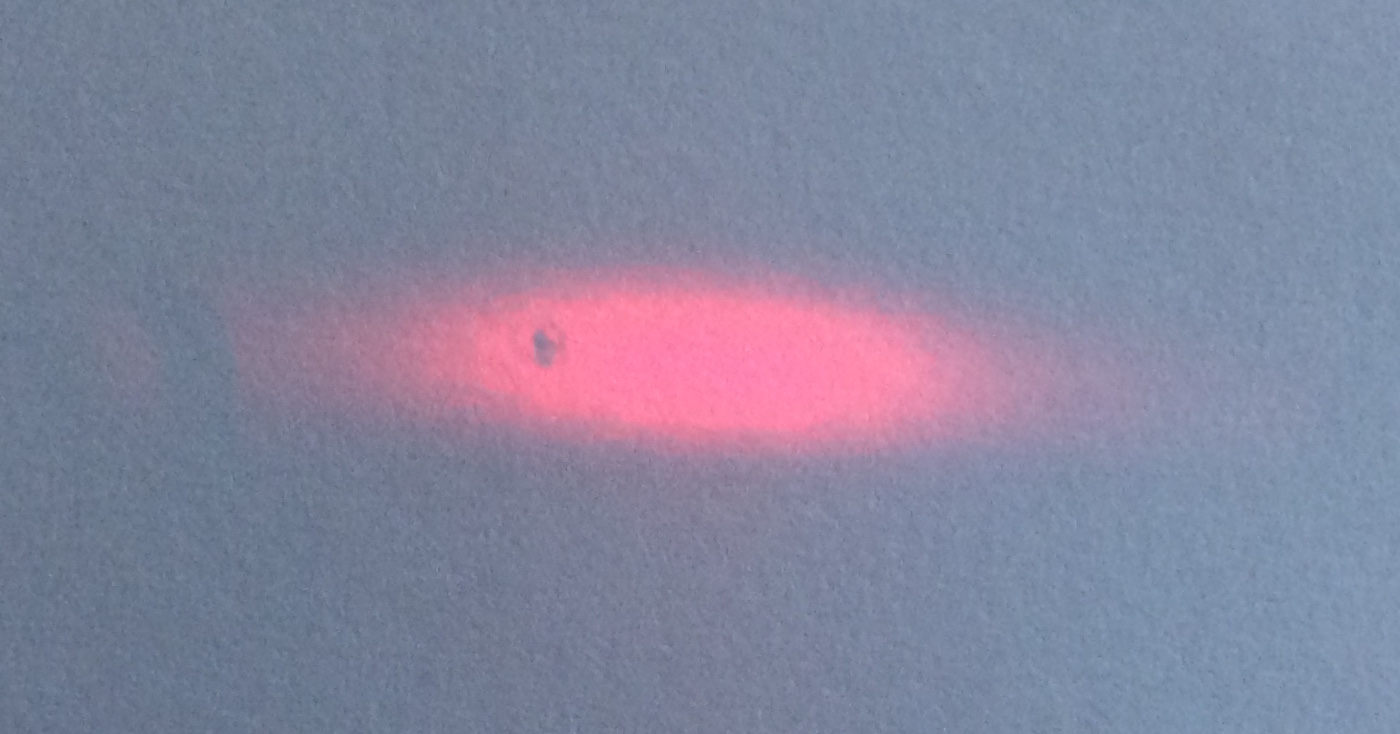
\includegraphics[width=0.49\textwidth]{laser/bilder/schwach.jpg}}\hfill
\subfigure[2.073 Volt Diodenspannung]
{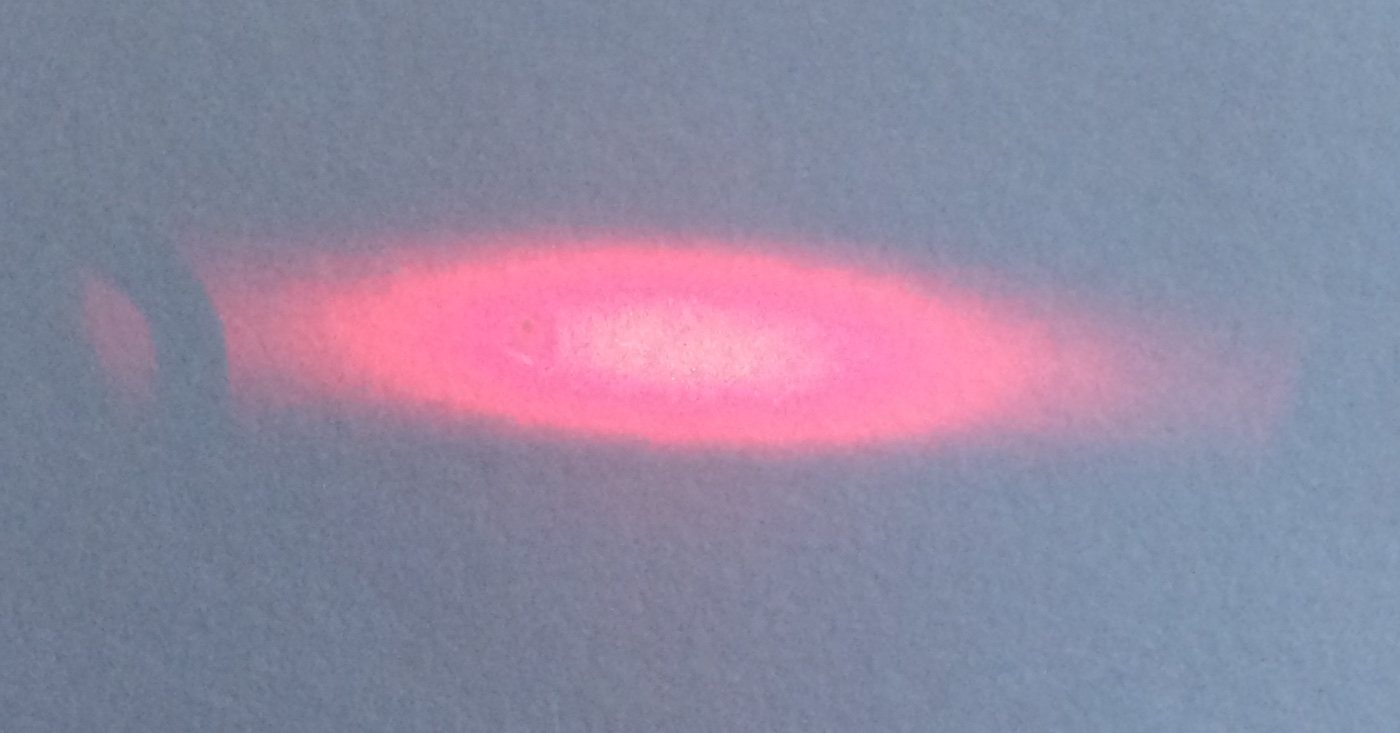
\includegraphics[width=0.49\textwidth]{laser/bilder/stark.jpg}}
\caption{Unterschied in der Laserstrahlst"arke beim "ubergang}
\label{fig:faecher}
\end{figure}

In diesen Abbildungen \ref{fig:faecher} ist ebenfalls sch"on zu sehen wie die 
Laserstrahlen in einem breiten F"acher abgegeben werden. Normalerweise werden 
die Laserstrahlen noch mittels einer Sammellinse geb"undelt. Dieser F"acher 
entsteht, weil die Laserdiode einen Kantenemitter ist. Das bedeutet, dass das 
Licht das Lasermedium an der Bruchkante nahe an der Oberfl"ache quer zum Strom 
verl"asst. Ein vereinfachter Schichtaufbau einer Laserdiode ist in 
Abbildung \ref{Laserdiodeaufbau} gut zu sehen. In den Abbildung 
\ref{fig:kennlinie} stellen wir die Leistung durch die Photodiode und den 
Strom durch die Laserdiode in Abh"angigkeit der Spannung "uber der Laserdiode 
dar. 
\begin{figure}
\centering
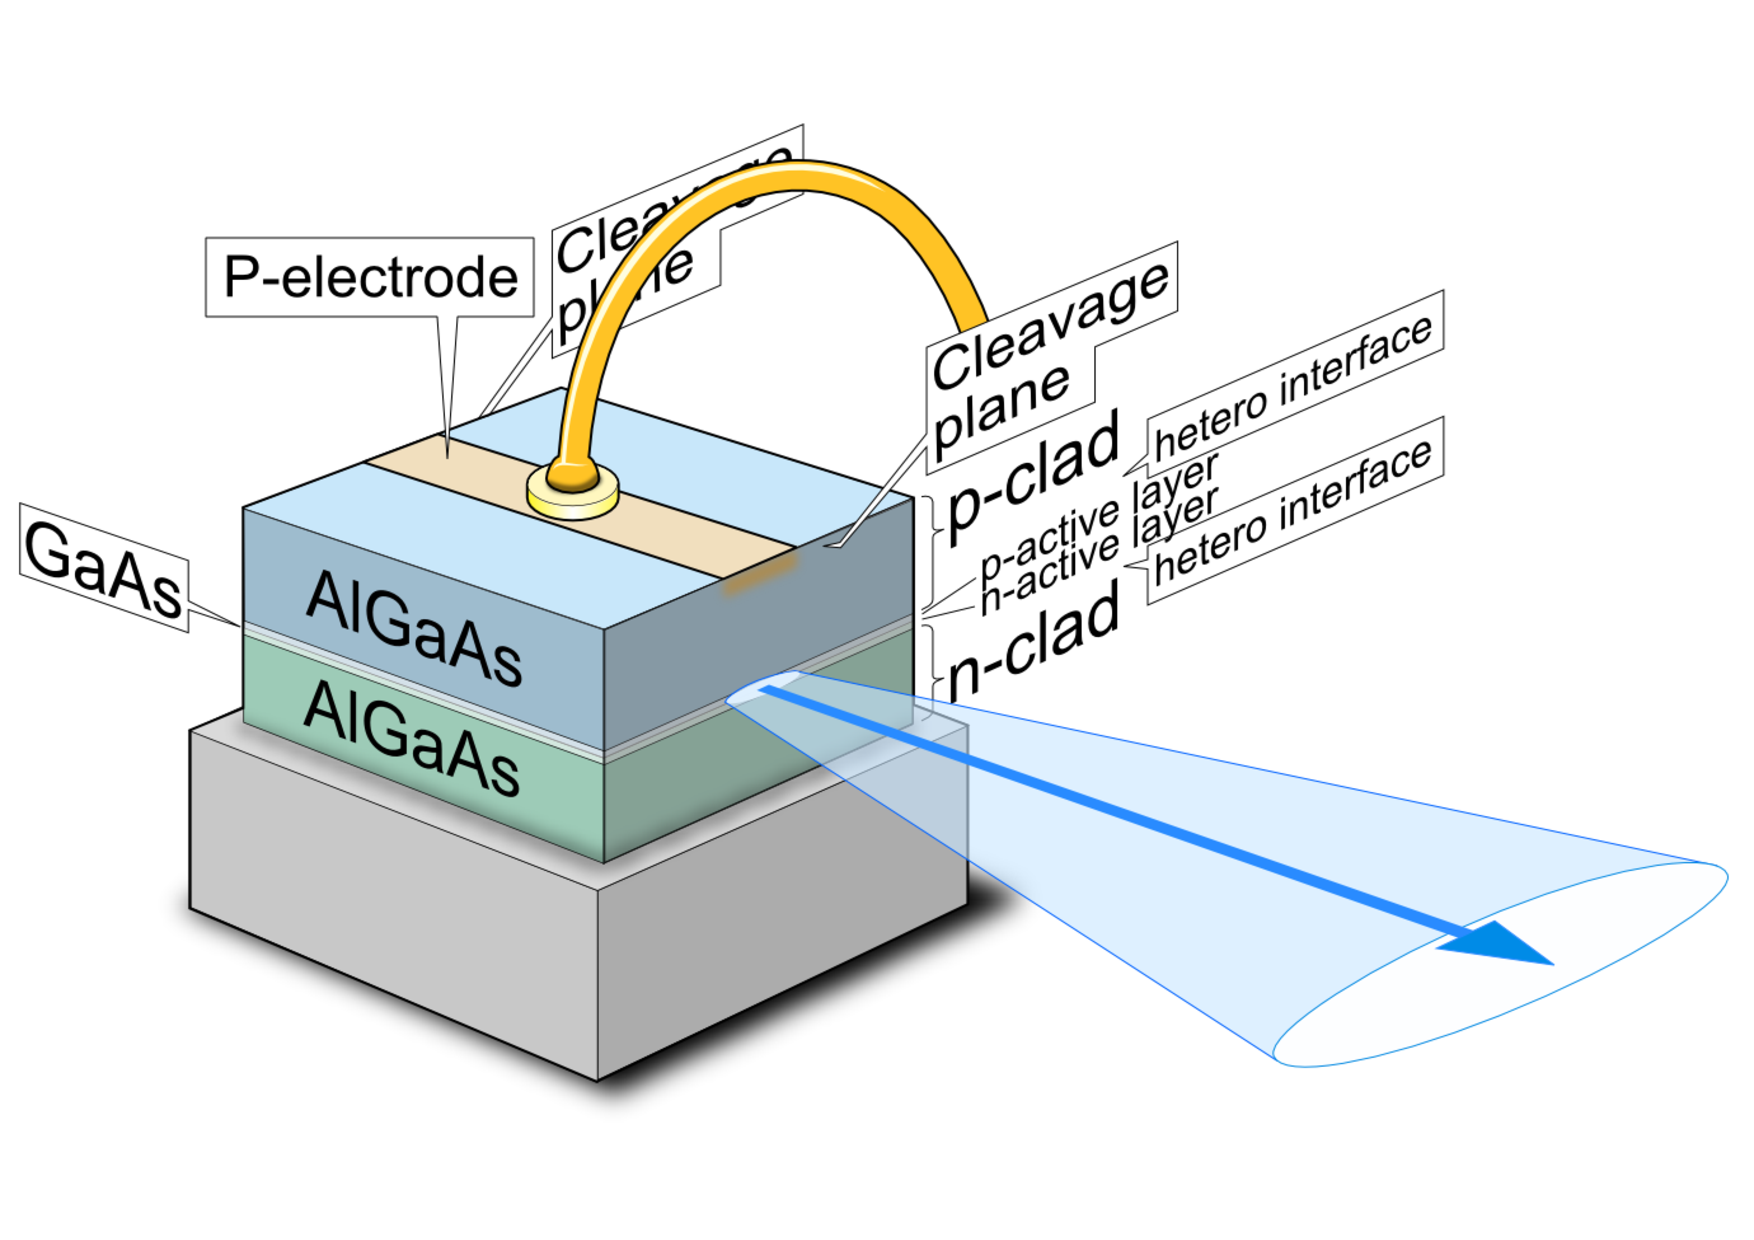
\includegraphics[width = 7cm]{laser/bilder/Diodenaufbau.pdf}
\caption{Vereinfachter Schichtaufbau des Laserdiodenchips (Kantenemitter)
\cite{WikiDiode}}
\label{Laserdiodeaufbau}
\end{figure}

\begin{figure}
\centering
\subfigure[Kennlinie Laserdiode]
{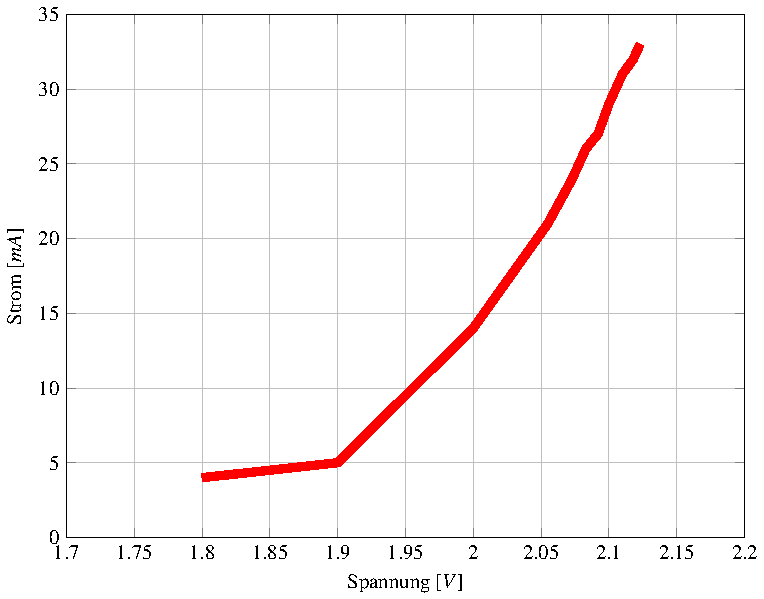
\includegraphics[width=0.49\textwidth]{laser/bilder/Dioden_Strom2.pdf}}\hfill
\subfigure[Kennlinie Photodiode]
{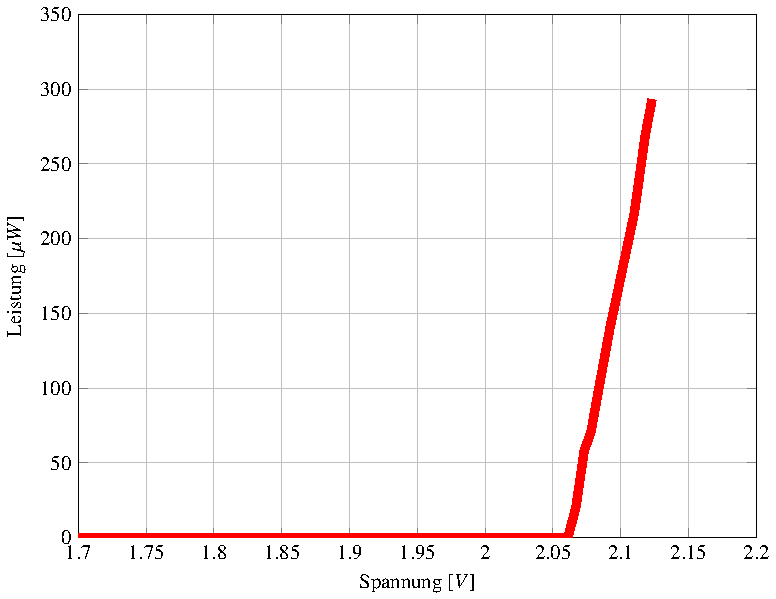
\includegraphics[width=0.49\textwidth]{laser/bilder/Dioden_Leistung2.pdf}}
\caption{In der Messung aufgenommene Kennlinie}
\label{fig:kennlinie}
\end{figure}

%Quelle ap-2015 und Wikipedia Laserdiode und Wikipedia LED


\section{Helium-Neon-Laser}
\label{He-Ne-Laser}
%------------------------------
%Quelle
% http://de.wikipedia.org/wiki/Helium-Neon-Laser, 31.M"arz 2015
% Laserphysik, Grundlagen und Anwendungen f"ur Ingenieure
%------------------------------

Der Helium-Neon-Laser war der erste Dauerstrichlaser und ebenfalls der erste 
realisierte Gaslaser. Zu Beginn wurde der Laser bei einer Wellenl"ange von 
1.15$\mu$m betrieben. Dies ist ausserhalb des sichtbaren Bereiches. Heute wird 
er haupts"achlich im sichtbaren Bereich betrieben. Die wichtigsten Linien sind 
die rote (632.8 nm), die gr"une (543.3 nm), die gelbe (594.1 nm) und die 
orange (611.8 nm).

Wegen der geringen Strahlverzerrung werden diese Lasermodelle als 
Ausrichtungsquellen mit hoher Strahlqualit"at oder als hochkoh"arente 
Laserquellen in der Holographie oder Interferometrie verwendet.

\subsection{Aufbau}
\label{He-Ne-Laser Aufbau}
Der Helium-Neon-Laser besteht aus einem d"unnen Glasr"ohrchen mit einem 
Durchmesser von ungef"ahr 1 mm und einigen dm L"ange. Es ist gef"ullt mit 
einem Helium-Neon-Gasgemisch. 
Dieses Gemisch steht unter einem Druck von ungef"ahr 100 Pa(=1mbar).
Die Partialdr"ucke stehen im Verh"altnis Helium/Neon = 10/1 f"ur eine 
Wellenl"ange von 1152 nm(infrarot),
beziehungsweise 5/1 f"ur eine Wellenl"ange von 633 nm(orange).
Die Abbildung \ref{HeNeLaserschema} zeigt den Aufbau.

Links und rechts von diesem Glasr"ohrchen befinden sich Resonatorspiegel.
Zus"atzlich zu diesen k"onnen auch noch Brewsterfenster eingebaut werden.
Brewsterfester sind planparallele Platten, die Licht mit einer bestimmten 
Polarisationsrichtung ohne Verluste durch Reflexion hin durchlassen. Somit 
gibt es nur einen durchgelassenen, keinen reflektierenden Strahl dieser 
Polarisationsrichtung. Licht mit dazu senkrechter Polarisation wird teilweise 
reflektiert.
Der Laser w"ahlt stets den Betriebszustand mit den geringsten Verlusten. Aus 
diesem Grund wird die "falsche" Polarit"at unterdr"uckt.

Die Spannungsversorung der Gasentladung muss einerseits zu Beginn die 
Z"undspannung von $10 - 15$ kV bereitstellen und anschliessend den 
Entladungsstrom begrenzen k"onnen, der nach der Z"undung fliesst.

\begin{figure}
\centering
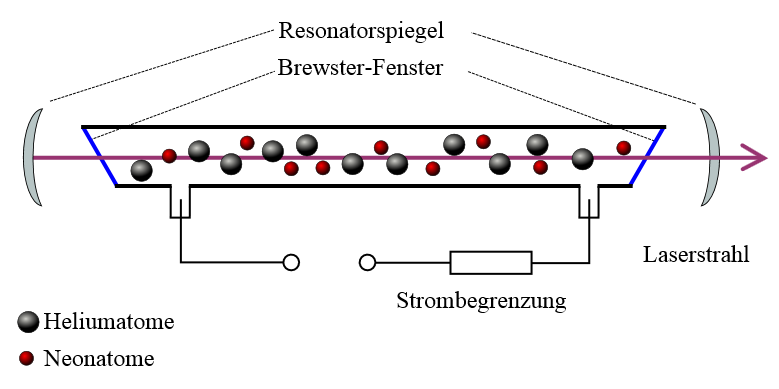
\includegraphics[width = 10cm]{laser/bilder/Laserschema.png}
%Quelle: „Henelaserschema“ von Ulfbastel - modifiziert austhumb|center|350px. Lizenziert unter GFDL "uber Wikimedia Commons - http://commons.wikimedia.org/wiki/File:Henelaserschema.svg#/media/File:Henelaserschema.svg
\caption{Helium-Neon-Laser Aufbau \cite{He-Ne-Laser-Aufbau}}
\label{HeNeLaserschema}
\end{figure}


%------------------------------
\subsection{Laservorgang}
Das Neon ist beim He-Ne-Laser das aktive Medium. Das Helium wird f"ur den 
Pumpprozess ben"otigt. 
Da das Helium noch eine hohe W"armeleitf"ahigkeit besitzt, dient es 
gleichzeitig auch zur K"uhlung des Gasgemisches.

Das Pumpen der Ne-Atome geschieht, wie in Abbildung \ref{Energieschema} 
dargestellt, durch die elektrischen Entladungen in einem 2 stufigen Prozess. 
Zuerst werden die Helium Atome durch Kollisionen mit den Elektronen aus der 
Gasentladung angeregt. Damit werden die He-Atome in die h"oherliegenden 
Energieniveaus gebracht.
Die Helium-Atome haben einen vergleichsweise langlebigen angeregten Zustand. 
Nun wird die gespeicherte Energie in den He-Atomen durch atomare Kollisionen 
auf die Ne-Atome "ubertragen. Dort wird die Besetzungsinversion zwischen 
energetisch hohen und tiefen Zust"anden erzeugt. Dies ist m"oglich, da die 
atomaren Niveaus von Helium und Neon ungef"ahr gleich gross sind.

Durch stimulierte Emission werden nun die Photonen mit der entsprechenden 
Energie/Frequenz frei. Das ist nun der altbekannte Laserbetrieb.

Die R"uckkehr in das unterste Energieniveau  gelingt durch spontane Emission 
und Rekombination an der Kapillarwand. Diese Tatsache ist daf"ur 
verantwortlich, dass der Durchmesser des Glasr"ohrchens nicht gr"osser als 1.5 
mm zu w"ahlen ist. 


\begin{figure}
\centering
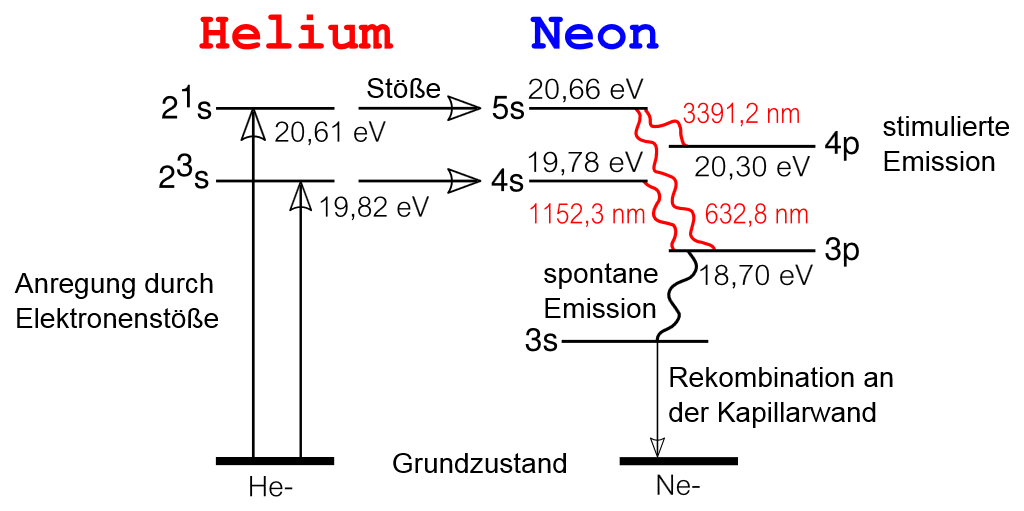
\includegraphics[width = 10cm]{laser/bilder/Energieschema.png}
%Quelle :„He-Ne-Laser-Energieschema“ von Bubinator - https://commons.wikimedia.org/wiki/File:He-ne-laser.svg. Lizenziert unter CC BY-SA 3.0 "uber Wikimedia Commons - http://commons.wikimedia.org/wiki/File:He-Ne-Laser-Energieschema.svg#/media/File:He-Ne-Laser-Energieschema.svg
\caption{Energieschema \cite{He-Ne-Laser-Energieschema}}
\label{Energieschema}
\end{figure}

\printbibliography[heading=subbibliography]

\end{refsection}

